\documentclass[times]{itmo-student-thesis}

%% Опции пакета:
%% - specification - если есть, генерируется задание, иначе не генерируется
%% - annotation - если есть, генерируется аннотация, иначе не генерируется
%% - times - делает все шрифтом Times New Roman, собирается с помощью xelatex
%% - languages={...} - устанавливает перечень используемых языков. По умолчанию это {english,russian}.
%%                     Последний из языков определяет текст основного документа.

%% Делает запятую в формулах более интеллектуальной, например:
%% $1,5x$ будет читаться как полтора икса, а не один запятая пять иксов.
%% Однако если написать $1, 5x$, то все будет как прежде.
\usepackage{icomma}

%% Один из пакетов, позволяющий делать таблицы на всю ширину текста.
\usepackage{tabularx}

\usepackage{xspace}

\usepackage{graphicx}
\graphicspath{{imgs/}}
\DeclareGraphicsExtensions{.png,.jpg}

%\usepackage[utf8]{inputenc}
%\usepackage{pgfplots}

%\usepgfplotslibrary{groupplots,dateplot}
%\usetikzlibrary{patterns,shapes.arrows}
%\pgfplotsset{compat=newest}

\newcommand{\alglambda}{${(1 + (\lambda , \lambda))}$\xspace}
\newcommand{\alglambdaf}{${(1 + (\lambda , \lambda))}$-ГА\xspace}


\newcommand{\oea}{\mbox{$(1 + 1)$-ЭА}\xspace}
\newcommand{\oplea}{\mbox{$(1+\lambda)$-ЭА}\xspace}
\newcommand{\mpoea}{\mbox{$(\mu+1)$-ЭА}\xspace}
\newcommand{\mplea}{\mbox{$(\mu+\lambda)$-ЭА}\xspace}
\newcommand{\mclea}{\mbox{$(\mu,\lambda)$-ЭА}\xspace}
\newcommand{\oclea}{\mbox{$(1,\lambda)$-ЭА}\xspace}
\newcommand{\ollga}{${(1 + (\lambda , \lambda))}$-ГА\xspace}

\newcommand{\onemax}{\textsc{OneMax}\xspace}
\newcommand{\leadingones}{\textsc{LeadingOnes}\xspace}
\newcommand{\om}{\textsc{OM}\xspace}
\newcommand{\jump}{\textsc{Jump}\xspace}
\newcommand{\N}{{\mathbb N}}
\newcommand{\R}{{\mathbb R}}
\newcommand{\eps}{\varepsilon}

\renewcommand{\binom}[2]{\mbox{$C^{#2}_{#1}$}}

\DeclareMathOperator{\Bin}{Bin}
\DeclareMathOperator{\Geom}{Geom}
\DeclareMathOperator{\pow}{pow}
\DeclareMathOperator*{\argmax}{arg\,max}
\DeclareMathOperator*{\argmin}{arg\,min}
%% Данные пакеты необязательны к использованию в бакалаврских/магистерских
%% Они нужны для иллюстративных целей
%% Начало
\usepackage{tikz}
\usetikzlibrary{arrows}
\usepackage{filecontents}

\begin{filecontents}{bachelor-thesis.bib}
@article{DoerrDE15,
  author = {Benjamin Doerr and
Carola Doerr and
Franziska Ebel},
  title = {From black-box complexity to designing new genetic algorithms},
  year = {2015},
  journal = {Theoretical Computer Science},
  optdoi = {10.1016/j.tcs.2014.11.028},
  optissn = {0304-3975},
  optnote = {Preliminary version in Proc.~of GECCO 2013},
  opturl = {http://dx.doi.org/10.1016/j.tcs.2014.11.028},
  pages = {87--104},
  volume = {567},
  langid = {english}
}

@inproceedings{AntipovDK19,
  author = {Denis Antipov and
Benjamin Doerr and
Vitalii Karavaev},
  title = {A tight runtime analysis for the {(1} + ({\(\lambda\)}, {\(\lambda\)}))
{GA} on {L}eading{O}nes},
  booktitle = {Foundations of Genetic Algorithms, {FOGA} 2019},
  year = {2019},
  pages = {169--182},
  publisher = {ACM},
  langid = {english}
}

@inproceedings{AntipovDK19,
  author = {Denis Antipov and
Benjamin Doerr and
Vitalii Karavaev},
  title = {A tight runtime analysis for the {(1} + ({\(\lambda\)}, {\(\lambda\)}))
{GA} on {L}eading{O}nes},
  booktitle = {Foundations of Genetic Algorithms, {FOGA} 2019},
  year = {2019},
  pages = {169--182},
  publisher = {ACM},
  langid = {english}
}

@inproceedings{BuzdalovD17,
  author = {Maxim Buzdalov and Benjamin Doerr},
  title = {Runtime analysis of the $(1+(\lambda,\lambda))$ genetic algorithm on random satisfiable 3-{CNF} formulas},
  booktitle = {Genetic and Evolutionary Computation Conference, {GECCO} 2017},
  year = {2017},
  optnote = {Full version available at \url{http://arxiv.org/abs/1704.04366}},
  pages = {1343-1350},
  publisher = {{ACM}},
  langid = {english}
}

@article{NeumannW07,
  author = {Frank Neumann and
Ingo Wegener},
  title = {Randomized local search, evolutionary algorithms, and the minimum
spanning tree problem},
  year = {2007},
  journal = {Theoretical Computer Science},
  optjournal = {Theor. Comput. Sci.},
  optnumber = {1},
  pages = {32--40},
  volume = {378},
  langid = {english}
}

@inproceedings{DoerrJW10,
  author = {Doerr, Benjamin and Johannsen, Daniel and Winzen, Carola},
  title = {Multiplicative drift analysis},
  booktitle = {Genetic and Evolutionary Computation Conference, GECCO 2010},
  year = {2010},
  optnote = {Best paper award},
  pages = {1449--1456},
  publisher = {ACM},
  langid = {english}
}

@inproceedings{AntipovBD20,
  author = {Denis Antipov and
Maxim Buzdalov and
Benjamin Doerr},
  title = {Fast mutation in crossover-based algorithms},
  booktitle = {Genetic and Evolutionary Computation Conference,
{GECCO} 2020},
  year = {2020},
  pages = {1268--1276},
  publisher = {{ACM}}
}

@inproceedings{DoerrG09,
  author = {Benjamin Doerr and Madeleine Theile},
  title = {Improved analysis methods for crossover-based algorithms},
  booktitle = {Genetic and Evolutionary Computation Conference,
{GECCO} 2009},
  year = {2009},
  pages = {247--254},
  publisher = {{ACM}}
}

@inproceedings{Dirk2014,
  author = {Dirk Sudholt},
  title = {Crossover speeds up building-block assembly},
  booktitle = {Genetic and Evolutionary Computation Conference,
{GECCO} 2012},
  year = {2012},
  pages = {689--702},
  publisher = {{ACM}}
}

@inproceedings{Crossover2008,
  author = {Benjamin Doerr and Edda Happ and Christian Klein},
  title = {Crossover can provably be useful in evolutionary computation},
  booktitle = {Genetic and Evolutionary Computation Conference,
{GECCO} 2008},
  year = {2008},
  pages = {539--546},
  publisher = {{Association for Computing Machinery}}
}

@article{DoerrD18,
  author = {Benjamin Doerr and Carola Doerr},
  title = {Optimal static and self-adjusting parameter choices for the (1+({\(\lambda\)},
{\(\lambda\)})) genetic algorithm},
  year = {2018},
  journal = {Algorithmica},
  optnumber = {5},
  pages = {1658--1709},
  volume = {80},
  langid = {english}
}

@inproceedings{GoldmanP14,
  author = {Brian W. Goldman and
William F. Punch},
  title = {Parameter-less population pyramid},
  booktitle = {Genetic and Evolutionary Computation Conference, {GECCO} 2014},
  year = {2014},
  optbooktitle = {Genetic and Evolutionary Computation Conference, {GECCO} '14, Vancouver,
BC, Canada, July 12-16, 2014},
  optdoi = {10.1145/2576768.2598350},
  opteditor = {Dirk V. Arnold},
  pages = {785--792},
  publisher = {{ACM}},
  langid = {english}
}

@inproceedings{ShiNW19,
  author    = {Feng Shi and
               Frank Neumann and
               Jianxin Wang},
  OPTeditor    = {Tobias Friedrich and
               Carola Doerr and
               Dirk V. Arnold},
  title     = {Runtime analysis of evolutionary algorithms for the depth restricted
               (1, 2)-minimum spanning tree problem},
  booktitle = {Foundations of Genetic Algorithms, {FOGA} 2019},
  pages     = {133--146},
  publisher = {{ACM}},
  year      = {2019},
  langid = {english}
}

@inproceedings{Witt05,
  author = {Carsten Witt},
  title = {Worst-case and average-case approximations by simple randomized search
Heuristics},
  booktitle = {Symposium on Theoretical Aspects of Computer
Science, {STACS} 2005},
  year = {2005},
  optbooktitle = {{STACS} 2005, 22nd Annual Symposium on Theoretical Aspects of Computer
Science, Stuttgart, Germany, February 24-26, 2005, Proceedings},
  optdoi = {10.1007/978-3-540-31856-9\_4},
  opteditor = {Volker Diekert and
Bruno Durand},
  optseries = {Lecture Notes in Computer Science},
  optvolume = {3404},
  pages = {44--56},
  publisher = {Springer},
  langid = {english}
}

@inproceedings{NeumannS19,
  author    = {Frank Neumann and
               Andrew M. Sutton},
  OPTeditor    = {Tobias Friedrich and
               Carola Doerr and
               Dirk V. Arnold},
  title     = {Runtime analysis of the {(1} + 1) evolutionary algorithm for the chance-constrained
               knapsack problem},
  booktitle = {Foundations of Genetic Algorithms, {FOGA} 2019},
  OPTbooktitle = {Proceedings of the 15th {ACM/SIGEVO} Conference on Foundations of
               Genetic Algorithms, {FOGA} 2019, Potsdam, Germany, August 27-29, 2019},
  pages     = {147--153},
  publisher = {{ACM}},
  year      = {2019},
  OPTdoi       = {10.1145/3299904.3340315},
  langid = {english}
}

@article{OlivetoHY09,
  author = {Pietro Simone Oliveto and
Jun He and
Xin Yao},
  title = {Analysis of the {(1+1)}-{EA} for finding approximate solutions to vertex
cover problems},
  year = {2009},
  journal = {{IEEE} Transactions on Evolutionary Computation},
  optnumber = {5},
  pages = {1006--1029},
  volume = {13},
  langid = {english}
}

@inproceedings{AntipovDK20,
  author = {Denis Antipov and Benjamin Doerr and Vitalii Karavaev},
  title = {The $(1 + (\lambda,\lambda))$ {GA} is even faster on multimodal problems},
  booktitle = {Genetic and Evolutionary Computation Conference, GECCO 2020},
  year = {2020},
  note = {To appear},
  optpages = {to appear},
  publisher = {{ACM}},
  langid = {english}
}

@inproceedings{Dang16,
  author = {Duc-Cuong Dang and Tobias Friedrich and Timo Kötzing and Martin S. Krejca},
  title = {Escaping local optima with diversity mechanisms and crossover},
  booktitle = {Genetic and Evolutionary Computation Conference, GECCO 2016},
  year = {2016},
  note = {To appear},
  optpages = {to appear},
  publisher = {{ACM}},
  langid = {english}
}

@inproceedings{Antipov2020,
  author = {Denis Antipov and Benjamin Doerr},
  title = {Runtime Analysis of a Heavy-Tailed $(1 + (\lambda,\lambda))$ Genetic Algorithm on Jump Functions},
  booktitle = {Parallel Problem Solving from Nature, {PPSN} 2020},
  year = {2020},
  pages = {545-559},
  publisher = {{Springer}},
  langid = {english}
}

@inproceedings{Doerr2011,
  author = {Benjamin Doerr},
  title = {Analyzing randomized search heuristics: tools from probability theory},
  booktitle = {Theory of Randomized Search Heuristics},
  year = {2011},
  pages = {1-20},
  publisher = {{World Scietific Publishing}},
  langid = {english}
}

@article{He00driftanalysis,
    author = {Jun He and Xin Yao},
    title = {Drift Analysis and Average Time Complexity of Evolutionary Algorithms},
    journal = {Artificial Intelligence},
    year = {2000},
    volume = {127},
    pages = {57--85},
    langid = {english}
}

@article{Cambridge2013,
    author = {Carsten Witt},
    title = {Tight Bounds on the Optimization Time of a Randomized Search Heuristic on Linear Functions},
    journal = {Combinatorics, Probability and Computing},
    year = {2013},
    volume = {22},
    pages = {294--318},
    langid = {english}
}

@inproceedings{MironovichB15,
  author = {Vladimir Mironovich and
Maxim Buzdalov},
  title = {Hard test generation for maximum flow algorithms with the fast crossover-based
evolutionary algorithm},
  booktitle = {Genetic and Evolutionary Computation Conference, {GECCO} 2015, Companion Material},
  year = {2015},
  pages = {1229--1232},
  langid = {english}
}

@book{Cormen09,
  author={Cormen, Thomas H and Leiserson, Charles E and Rivest, Ronald L and Stein, Clifford},
  title={Introduction to algorithms},
  year={2009},
  publisher={MIT press},
  langid = {english}
}

@article{Skobtsov08,
  title={Основы эволюционных вычислений},
  author={Скобцов, Юрий Александрович},
  year={2008},
  publisher={ДонНТУ},
  langid      = {russian}
}

@article{Gmurman14,
  title={Теория вероятностей и математическая статистика},
  author={Гмурман, Владимир Ефимович and Гмурман, Владимир Владимирович and Колосова, Татьяна Владимировна},
  year={2014},
  publisher={Общество с ограниченной ответственностью Издательство ЮРАЙТ},
  langid      = {russian}
}

@book{Kudryavtsev03,
  title={Сборник задач по математическому анализу},
  author={Кудрявцев, Лев Дмитриевич and Кутасов, АД and Чехлов, ВИ and Шабунин, МИ},
  year={2003},
  publisher={Физматлит},
  langid      = {russian}
}

@article{Doerr18,
  title = {An elementary analysis of the probability that a binomial random variable exceeds its expectation},
  journal = {Statistics & Probability Letters},
  volume = {139},
  pages = {67-74},
  year = {2018},
  OPTissn = {0167-7152},
  OPTdoi = {https://doi.org/10.1016/j.spl.2018.03.016},
  OPTurl = {https://www.sciencedirect.com/science/article/pii/S0167715218301366},
  author = {Benjamin Doerr},
}

@InCollection{Doerr20bookchapter,
  author="Doerr, Benjamin",
  editor="Doerr, Benjamin
  and Neumann, Frank",
  title="Probabilistic tools for the analysis of randomized optimization heuristics",
  bookTitle="Theory of Evolutionary Computation: Recent Developments in Discrete Optimization",
  year="2020",
  publisher="Springer",
  OPTaddress="Cham",
  pages="1--87",
  OPTisbn="978-3-030-29414-4",
  OPTdoi="10.1007/978-3-030-29414-4_1",
  OPTurl="https://doi.org/10.1007/978-3-030-29414-4_1",
    vgwort = {p2: 2942*86/1500=168.67=169},
  OPTnote = {Also available at \url{https://arxiv.org/abs/1801.06733}}
}

@inproceedings{DoerrJW10,
  author    = {Doerr, Benjamin and Johannsen, Daniel and Winzen, Carola},
  title     = {Multiplicative drift analysis},
  booktitle = {Genetic and Evolutionary Computation Conference, GECCO 2010},
  year      = {2010},
  pages     = {1449--1456},
  optnote = {Best paper award},
  publisher = {ACM}
}

\end{filecontents}
%% Конец

%% Указываем файл с библиографией.
\addbibresource{bachelor-thesis.bib}

\begin{document}

\studygroup{M3435}
\title{Анализ генетического алгоритма (1 + (лямбда, лямбда)) на задаче максимального разреза графа}
\author{Черноокая Виктория Александровна}{Черноокая В.А.}
\supervisor{Антипов Денис Сергеевич}{Антипов Д.С.}{PhD}{}
\publishyear{2022}
%% Дата выдачи задания. Можно не указывать, тогда надо будет заполнить от руки.
\startdate{01}{сентября}{2018}
%% Срок сдачи студентом работы. Можно не указывать, тогда надо будет заполнить от руки.
\finishdate{31}{мая}{2019}
%% Дата защиты. Можно не указывать, тогда надо будет заполнить от руки.
%%\defencedate{15}{июня}{2019}

%%\addconsultant{Белашенков Н.Р.}{канд. физ.-мат. наук, без звания}
%%\addconsultant{Беззубик В.В.}{без степени, с велкиим званием}

\secretary{Павлова О.Н.}

%% Задание
%%% Техническое задание и исходные данные к работе
\technicalspec{Требуется разработать стилевой файл для системы \LaTeX, позволяющий оформлять бакалаврские работы и магистерские диссертации
на кафедре компьютерных технологий Университета ИТМО. Стилевой файл должен генерировать титульную страницу пояснительной записки,
задание, аннотацию и содержательную часть пояснительной записк. Первые три документа должны максимально близко соответствовать шаблонам документов,
принятым в настоящий момент на кафедре, в то время как содержательная часть должна максимально близко соответствовать ГОСТ~7.0.11-2011
на диссертацию.}

%%% Содержание выпускной квалификационной работы (перечень подлежащих разработке вопросов)
\plannedcontents{Пояснительная записка должна демонстрировать использование наиболее типичных конструкций, возникающих при составлении
пояснительной записки (перечисления, рисунки, таблицы, листинги, псевдокод), при этом должна быть составлена так, что демонстрируется
корректность работы стилевого файла. В частности, записка должна содержать не менее двух приложений (для демонстрации нумерации рисунков и таблиц
по приложениям согласно ГОСТ) и не менее десяти элементов нумерованного перечисления первого уровня вложенности (для демонстрации корректности
используемого при нумерации набора русских букв).}

%%% Исходные материалы и пособия
\plannedsources{\begin{enumerate}
    \item ГОСТ~7.0.11-2011 <<Диссертация и автореферат диссертации>>;
    \item С.М. Львовский. Набор и верстка в системе \LaTeX;
    \item предыдущий комплект стилевых файлов, использовавшийся на кафедре компьютерных технологий.
\end{enumerate}}

%%% Цель исследования
\researchaim{Разработка удобного стилевого файла \LaTeX
             для бакалавров и магистров кафедры компьютерных технологий.}

%%% Задачи, решаемые в ВКР
\researchtargets{\begin{enumerate}
    \item обеспечение соответствия титульной страницы, задания и аннотации шаблонам, принятым в настоящее время на кафедре;
    \item обеспечение соответствия содержательной части пояснительной записки требованиям ГОСТ~7.0.11-2011 <<Диссертация и автореферат диссертации>>;
    \item обеспечение относительного удобства в использовании~--- указание данных об авторе и научном руководителе один раз и в одном месте, автоматический подсчет числа тех или иных источников.
\end{enumerate}}

%%% Использование современных пакетов компьютерных программ и технологий
\addadvancedsoftware{Пакет \texttt{tabularx} для чуть более продвинутых таблиц}{\ref{sec:tables}, Приложения~\ref{sec:app:1}, \ref{sec:app:2}}
\addadvancedsoftware{Пакет \texttt{biblatex} и программное средство \texttt{biber}}{Список использованных источников}

%%% Краткая характеристика полученных результатов
\researchsummary{Получился, надо сказать, практически неплохой стилевик. В 2015--2018 годах
его уже использовали некоторые бакалавры и магистры. Надеюсь на продолжение.}

%%% Гранты, полученные при выполнении работы
\researchfunding{Автор разрабатывал этот стилевик исключительно за свой счет и на
добровольных началах. Однако значительная его часть была бы невозможна, если бы
автор не написал в свое время кандидатскую диссертацию в \LaTeX,
а также не отвечал за формирование кучи научно-технических отчетов по гранту,
известному как <<5-в-100>>, что происходило при государственной финансовой поддержке
ведущих университетов Российской Федерации (субсидия 074-U01).}

%%% Наличие публикаций и выступлений на конференциях по теме выпускной работы
\researchpublications{По теме этой работы я (к счастью!) ничего не публиковал.
\begin{refsection}
Однако покажу, как можно ссылаться на свои публикации из списка литературы:
\nocite{example-english, example-russian}
\printannobibliography
\end{refsection}
}

%% Эта команда генерирует титульный лист и аннотацию.
\maketitle{Бакалавр}

%% Оглавление
\tableofcontents

%% Макрос для введения. Совместим со старым стилевиком.
\startprefacepage
Эволюционные вычисления являются достаточно общим термином, который содержит в себе множество похожих между собой техник.
Принцип эволюционного программирования состоит в имитации естественного отбора~\cite{Skobtsov08}.
Эволюционные алгоритмы --- такие алгоритмы оптимизации, в основном использующиеся для решения сложных задач ($NP$ - трудных) на практике.
Для этих задач не существует детерминированного алгоритма, решающего задачу за полиномиальное время.
В текущих реалиях, если только не $P = NP$, лучшее решение найти не представляется возможным, поэтому эволюционные алгоритмы находят достаточно хорошее решение за приемлемое время работы.

Генетический алгоритм \alglambda является одним из относительно недавно разработанных алгоритмов в области эволюционных вычислений. Одним из важных отличий его от других эволюционных алгоритмов является наличие фазы скрещивания.
Уже проводился анализ этого алгоритма на других задачах.
Например, было выявлено, что если размер потомства $\lambda$ немного меньше, чем $\Theta(\sqrt{\log(n)})$, теоретическая оценка времени работы алгоритма на задаче \onemax равна $O(n\sqrt{\log(n)})$~\cite{DoerrD18}, а это меньше времени любого эволюционного алгоритма, использующего только операторы мутации.
В работах ~\cite{DoerrD18} и~\cite{AntipovBD20} также анализировалась работа этого алгоритма на \onemax и было показано, что если параметр $\lambda$ выбирается динамически, то можно достичь времени работы $\Theta(n)$, лучшего на данный момент среди всех алгоритмов.
Для другой, популярной для исследований, модельной задачи  \leadingones был получен результат, показывающий, что ожидаемое время работы генетического алгоритма \alglambda схоже с эволюционным алгоритмом $(1+1)$~\cite{AntipovDK19}.

Несмотря на то, что уже были получены теоретические результаты анализа работы генетического алгоритма \alglambda для модельных функций, показывающие его преимущество, для практических задач результатов получено сравнительно мало.
В частности в работах ~\cite{BuzdalovD17, GoldmanP14} представлены оценки на задаче MAX3-SAT.
Помимо этого также известны результаты исследований для функций RoyalRoad~\cite{DoerrDE15} и некоторого числа комбинаторных задач~\cite{MironovichB15}.

За счет своей эффективности, доказанной экспериментально, эволюционные алгоритмы часто применяются на практике.
Но, к сожалению, на данный момент мы не обладаем достаточной информацией с теоретической точки зрения об их рабочих принципах.
Этот факт мешает подбирать для каждой конкретной задачи самый оптимальный алгоритм.

Цель данной работы --- улучшить понимание рабочих принципов эволюционных алгоритмов на задачах с графами.
Для достижения этой цели мы исследуем то, как различные эволюционные алгоритмы решают задачу о поиске максимального разреза графа, а точнее, находят приближение к нему.
В данной работе впервые анализируется работа \alglambdaf на $NP$-трудной задаче на графах.
Результаты помогут лучше понять специфику рабочих принципов алгоритмов и позволят в дальнейшем продолжить исследования на $NP$-трудных задачах на графах.

Так как для произвольного графа неизвестно заранее, какое максимальное число ребер может быть <<разрезано>>, то будем оценивать время работы эволюционных алгоритмов с условием, что должна быть <<разрезана>> хотя бы половина ребер.
Для разных типов графов такое решение может быть по-разному близко к оптимальному.
Например, для полных графов (для которых в данной работе будет приведена теоретическая оценка времени работы) мы можем <<разрезать>> максимум $\lfloor\frac{1}{2} |E| (1 + \frac{1}{n-1})\rfloor$ ребер.
Исходя из этого можно сказать, что решение с половиной <<разрезанных>> ребер --- это достаточно хорошая аппроксимация оптимального решения с точностью до множителя $1 + o(1)$.
Для двудольного же графа мы можем <<разрезать>> все ребра, если положим доли по разные стороны от разреза.
То есть для таких типов графов при разрезе половины ребер мы получаем решение, которое в два раза хуже оптимального.

В Главе 1 подробно описывается область исследования, которая включает в себя описание популярных эволюционных алгоритмов, основанных на мутации:
\begin{itemize}
  \item Random Local Search (RLS);
  \item \oea со стандартным оператором мутации;
  \item \oea с выбором вероятности по степенному закону.
\end{itemize}
А также описание задачи поиска максимального разреза графа и генетического алгоритма \alglambda.
Далее, в Главе 2 приводится теоретическая оценка времени работы предложенного алгоритма на полных графах, а также сравнение с ожидаемым временем работы других эволюционных алгоритмов, перечисленных выше.
В Главе 3 описываются критерии для получения эмпирической оценки и результаты выполнения известных эволюционных алгоритмов, включая генетический алгоритм \alglambda на полных, полных двудольных и случайных графах, а также сравнение применения алгоритмов на практике.

%% Начало содержательной части.
\chapter{Применение генетического алгоритма \alglambda на задаче поиска максимального разреза графа}

%% Так помечается начало обзора.
\startrelatedwork
В данной главе описываются эволюционные алгоритмы Random Local Search, \oea, генетический алгоритм \alglambda и постановка исследуемой задачи, а именно поиска максимального разреза графа.
Также сформулированны условия для получения теоретической и эмпирической оценки применения алгоритма \alglambda на задаче максимального разреза графа.
%% Так помечается конец обзора.
\finishrelatedwork

\section{Эволюционные алгоритмы, основанные на мутации}
В данной работе сравнивается работа \alglambdaf с другими популярными эволюционными алгоритмами, основанными на мутации:
\begin{itemize}
  \item Random Local Search (RLS);
  \item \oea со стандартным оператором мутации;
  \item \oea с выбором вероятности по степенному закону.
\end{itemize}

Данные алгоритмы работают по схожему принципу: хранят в себе родительскую особь, далее с помощью оператора мутации получается один потомок, который в случае улучшения значения функции приспособленности заменяет родителя.

Random Local Search --- достаточно популярный эволюционный алгоритм, основанный на мутации. На каждой итерации алгоритма инвертируется один случайный бит в разбиении $x$, полученное разбиение $x'$ заменяет родителя, если значение функции приспособленности не ухудшилось.

Далее рассмотрим \oea с различными типами мутации. В случае стандартной битовой мутации каждый бит в разбиении $x$ инвертируется с вероятностью $\frac{1}{n}$.
Полученный мутант заменяет родителя $x$, если улучшает функцию приспособленности.
Этот алгоритм уже может переносить несколько вершин из одного множества в другое.

Так как число инвертированных бит имеет биномиальное распределение, то математическое ожидание числа инвертированных бит равно единице.
Следовательно, данный алгоритм на этой задаче не сильно отличается от рассмотренного ранее RLS.

Следующим рассмотрим оператор мутации с выбором вероятности по степенному закону. На фазе мутации выбирается число $\lambda \in [1..n]$ из распределения с <<тяжелым хвостом>> $pow(\beta, n)$, что означает, что  вероятность выбрать число из $[1..n]$ пропорциональна $\lambda^{-\beta}$, где $\beta \in (1; 2)$ --- константный параметр.
Далее каждый символ заменяется с вероятностью $\frac{\lambda}{n}$. Такой алгоритм работает значительно лучше на многих сложных задачах.

\section{Генетический алгоритм \alglambda}

Генетический алгоритм \alglambda(далее \alglambdaf)~--- относительно недавно разработанный эволюционный алгоритм, минимизирующий функцию приспособленности $f(x)~:~\{0, 1\}^n \rightarrow \R$ и содержайщий в себе 3 главных параметра:
\begin{itemize}
   \item размер популяции $\lambda \in \N$;
   \item вероятность мутации $p \in [0, 1]$;
   \item смещённость скрещивания $c \in [0, 1]$.
\end{itemize}
\alglambdaf работает с одной родительской особью $x$, которая обычно инициализируется случайной битовой строкой длины $n$, где $n$ - размер задачи. В нашем случае особь инициализируется строкой из нулей. Затем проходят итерации, каждая из которых состоит из двух фаз: мутации и скрещивания~\cite{DoerrDE15}.

На этапе мутации алгоритм сначала выбирает силу мутации $\ell$ из биномиального распределения $\Bin(n, p)$ с $n$ испытаниями и вероятностью успеха $p$. В алгоритме \oea в фазе мутации мы имеем $p = \frac{1}{n}$, но поскольку мы стремимся к более быстрому результату, то обычно рассматривают вероятность $p$, превышающую $\frac{1}{n}$.
После этого создается $\lambda$ потомков, каждый путем инвертирования $\ell$ случайных бит родителя. То есть выбираем набор из $\ell$ различных позиций в $[n]$ случайным образом и создаем потомка, инвертировав битовые значения в этих позициях.
Все эти потомки находятся на одинаковом расстоянии от родителя.
На промежуточном этапе отбора потомок с наилучшим значением функции приспособленности выбирается победителем мутации для дальнейшего участия в фазе скрещивания. Если таких несколько, то победитель выбирается равномерно случайным образом среди претендентов.
Обозначим этого потомка как $x'$.

Далее следует фаза скрещивания. Снова создается $\lambda$ потомков. На этот раз каждый бит потомка берется из победителя мутации с вероятностью $c$ и из родителя с вероятностью $1 - c$. Победитель скрещивания $y$ выбирается тем же способом, как и на фазе мутации. В конце итерации происходит отбор или фаза выбора, где происходит сравнение значений функции приспособленности родителя $x$ и победителя скрещивания $y$.
Родитель заменяется особью-победителем $y$ фазы скрещивания, если значение $f(y)$ не хуже $f(x)$. Псевдокод алгоритма представлен в Листинге 1.

\begin{algorithm}[h]
\caption{Псевдокод \alglambdaf, максимизируещего $f$}\label{ollgaMin}
\begin{algorithmic}
	\State$x \gets $ \textsc{случайная последовательность бит длины} $n$
	\For{$t \gets [1, 2, 3...]$}
		\State \textsc{Выбрать} $\ell$ \textsc{из} $\Bin\left(n, p\right)$ \Comment Фаза мутации
      		\For{$i \in [1..\lambda]$}
         		\State$x^{(i)} \gets$ \textsc{копия} $x$ \textsc{с инвертированными} $\ell$ \textsc{битами, взятыми из равномерного распределения}
         	\EndFor
	     	\State $x' \gets \argmax_{z \in \{x^{(1)}, \dots, x^{(\lambda)}\}}f(z)$

		\For{$i \in [1..\lambda]$} \Comment Фаза срещивания
	          	\State $y^{(i)} \gets$ \textsc{каждый бит с вероятностью $c$ берётся из $x'$ иначе из $x$}
		\EndFor
	      	\State $y \gets \argmax_{z \in \{y^{(1)}, \dots, y^{(\lambda)}\} }f(z)$

		\If{$f(y) \ge f(x)$} \Comment Отбор
			\State $x \gets y$
		\EndIf
	\EndFor
\end{algorithmic}
\end{algorithm}

Алгоритм зависит от размера популяции $\lambda \in \N$ и вероятностей мутации и скрещивания $p, c \in [0, 1]$.
Без доказательства заметим, что алгоритм не сходится к оптимальному решению, когда $p = 0$ или $c = 0$, или $p = c = 1$. В обоих случаях на стадии скрещивания никогда не создается особь, отличная от изначальной.
Для всех остальных случаев он в конце концов находит (и сохраняет) оптимум.
При $c = 1$ на фазе скрещивания получается победитель мутации, что исключает влияние фазы скрещивания и \alglambdaf сводится к \oplea.
В частности, для $c = 1, p = \frac{1}{n}$ и $\lambda = 1$ алгоритм является \oea.
Во всех остальных случаях $0 < c < 1$ результат итерации алгоритма \alglambdaf зависит от фазы скрещивания.
Ее роль на данный момент еще недостаточно хорошо изучена, но уже существуют работы~\cite{Crossover2008, Dirk2014, Dang16, DoerrG09}, где описываются примеры, когда скрещивание улучшает работу алгоритма.

Поскольку для многих эволюционных алгоритмов, основанных на мутациях, вероятность мутации $\frac{1}{n}$ является рекомендуемым выбором~\cite{DoerrDE15} (и иногда доказуемо  оптимальным~\cite{Cambridge2013}), то следует использовать алгоритм \alglambdaf с $p, c$, удовлетворяющим $pc = \frac{1}{n}$.
Из интуитивных соображений в ~\cite{DoerrDE15} было предложено использовать такое соотношение параметров размера задачи $n$ и размера популяции $\lambda$:
\begin{itemize}
 \item $p = \frac{\lambda}{n}$;
 \item $c = \frac{1}{\lambda}$.
 \end{itemize}
Также такое соотношение параметров показало свою эффективность и было оптимальным на других анализируемых задачах, таких как \onemax~\cite{DoerrDE15}, \leadingones~\cite{AntipovDK19} и MAX-3SAT~\cite{BuzdalovD17}). В данной работе также используются предложенные соотношения параметров.


\section{Задача о максимальном разрезе графа}

Смысл задачи о максимальном разрезе графа --- для заданного неориентированного графа без петель и паралельных ребер $G = (V, E)$ с множеством вершин $V$ и ребер $E$ разбить множество вершин на два непересекающихся подмножества $V_1$ и $V_2$ так, что число <<разрезанных>> ребер было максимально и $V_1 \cup V_2 = V$.
 Ребро $(v, u) \in E$ назвается <<разрезанным>>, если инцидентные ему вершины находятся в разных подмножествах $V_1$ и $V_2$, то есть $v \in V_1 \cap u \in V_2$ или $v \in V_2 \cap u \in V_1$.

$P$ --- разбиение множества $V$ на два подмножества $V_1$ и $V_2$.
Представим его в виде битовой строки, где $i$-ый бит равен нулю, если $v_i \in V_1$, и единице, если $v_i \in V_2$.
Определим функцию  $Cut$ от разбиения $P$ :
\begin{align*}
   Cut(P) = |\{e = (v_1, v_2) \in E ~:~ v_1 \in V_1 \cap v_2 \in V_2\}|.
\end{align*}
Неформально говоря, это число <<разрезанных>> ребер.

Задача является $NP$-трудной, что в текущих реалиях означает, что не существует детерминированного алгоритма, решающего задачу за полиномиальное время. Поэтому на практике для нахождения достаточно хороших решений этой задачи часто используются эволюционные алгоритмы.
Обычно это нетривиальная задача, так как мы не можем заранее знать, сколько ребем мы можем <<разрезать>>. Например, для полного графа $K_n$ с четным $n$ оптимальным разбиением является то, которое разбивает вершины на два подмножества размером $\frac{n}{2}$. В этом случае мы разрезаем $\frac{n^2}{4}$ ребер, что чуть больше половины всех $\frac{n(n-1)}{2}$ ребер. В то же время для двудольных графов всегда существует решение, разрезающее все ребра. Следовательно, эволюционный алгоритм не может заранее знать, насколько он близок к оптимальному решению, и поэтому часто используется такой критерий остановки, при котором алгоритм завершает работу, если разрезана хотя бы половина ребер.

Ранее проводились исследования работы других эволюционных алгоритмов на данной задаче с таким условием остановки, однако нет опубликованных результатов.
В данной работе впервые проводится анализ \alglambdaf на задаче о максимальном разрезе, а также в целом на NP-трудной задаче на графах.

\chapterconclusion
В данной главе был сформулирован алгоритм \alglambdaf, а также задача, используемая для анализа времени работы на нем. Сформулированны и предложены оптимальные параметры для генетического алгоритма, а также затронуто сравнение реализации \alglambdaf с другими существующими эволюционными алгоритмами.

\chapter{Теоретическая оценка времени работы алгоритма на полных графах}
Теоретических оценок для задачи максимального разреза графа на данный момент не существует, поэтому целесообразно начать исследования в этой области с одного класса графов.
В данной главе приводится теоретическая оценка времени работы эволюционных алгоритмов RLS, \oea со стандартным оператором мутации и с оператором мутации с выбором вероятности по степенному закону, а также \alglambdaf на задаче поиска максимального разреза графа для полных графов.
Для этого типа графа, учитывая описанный ранее критерий остановки, алгоритм заканчивает работу, когда находит решение, очень близкое к оптимальному.

\section{Используемые математические результаты}

В приведенном теоретическом анализе часто используются границы Чернова в мультипликативной форме, формулировку и доказательство которых можно найти, например, в~\cite{Doerr20bookchapter} (Теоремы 1.10.1 и 1.10.5).

\begin{lemma}\label{lem:chernoff}
  Пусть случайная величина $X$ следует биномальному распределению $\Bin(n, p)$. Тогда для любой $\delta > 0$ верно, что
  \begin{align*}
    \Pr[X \ge (1 + \delta)E[X]] \le \exp\left(-\frac{\min\{\delta, \delta^2\}E[X]}{3}\right).
  \end{align*}
  Также для любой $\delta \in (0, 1)$ верно, что
  \begin{align*}
    \Pr[X \le (1 - \delta)E[X]] \le \exp\left(-\frac{\delta^2 E[X]}{2}\right).
  \end{align*}
\end{lemma}

Также используется мультипликативная теорема о сносе, впервые предложенная в~\cite{DoerrJW10}.

\begin{theorem}\label{thm:mult-drift}
  Пусть дано некоторое конечное множество положительных чисел $S$ с минимальным значением $s_{\min}$ и пусть дан случайный процесс $\{X_t\}_{t \in \N}$, принимающий значения из $S \cup \{0\}$. Пусть также $T$ есть самый первый момент времени, когда $X_t = 0$. Если существует $\delta > 0$ такая, что для всех $s \in S$
  \[
    E\left[X_t - X_{t + 1} \mid X_t = s\right] \ge \delta s,
  \]
  тогда для всех возможных $s$ также выполнено
  \[
    E[T \mid X_0 = s] \le \frac{1 + \ln(s_0/s_{\min})}{\delta}.
  \]
\end{theorem}

\section{Анализ эволюционных алгоритмов, основанных на мутации}
Необходимо оценить ожидаемое время, то есть число вычислений функции приспособленности, за которое разные эволюционные алгоритмы найдут разрез, в котором хотя бы половина общего числа ребер <<разрезаны>>.

Всего ребер в полном графе $\frac{n(n-1)}{2}$, где $n$ --- число вершин в графе.
Соответственно необходимо найти такое разбиение, что разрезаных ребер $\lceil \frac{n(n-1)}{4} \rceil$.
Обозначим $m_{\text{left}}$ и $m_{\text{right}}$ как число вершин по левую и по правую сторону от разреза соответственно. То есть $m_{\text{left}}$ есть число нулей в разбиении $P$, а $m_{\text{right}}$ есть число единиц в нем.
Обозначим $m = \min\{m_{\text{left}}, m_{\text{right}}\}$.
Тогда число <<разрезанных>> ребер в такой ситуации $m(n-m)$. Для определения момента времени, когда алгоритм заканчивает работу введем слудеющую лумму.

\begin{lemma}
  Хотя бы половина ребер в полном графе разрезана тогда и только тогда, когда $m \ge \frac{n - \sqrt{n}}{2}$, если $\frac{n(n - 1)}{2}$ -- четное, и когда $m \ge \frac{n - \sqrt{n - 2}}{2}$ в ином случае. Достаточным условием для разреза половины ребер является
  \[
    m \ge \frac{n - \sqrt{n - 2}}{2}.
  \]
\end{lemma}

\begin{proof}
  Рассмотрим два случая, когда число ребер в полном графе четное и нечетное соответственно.

  Пусть $\frac{n(n-1)}{2}$ четное, то есть $\lceil \frac{n(n-1)}{4} \rceil = \frac{n(n-1)}{4}$.
  Тогда оценим необходимое значение $m$ :
  $$
    m(n-m) \ge \frac{n(n-1)}{4}.
  $$

  Используя методы решения квадратных неравенств получаем промежуток значений:
  $$
  m \in \left[\frac{n - \sqrt{n}}{2}, \frac{n + \sqrt{n}}{2}\right].
  $$

  Теперь рассмотрим, если $\frac{n(n-1)}{2}$ нечетное, следовательно $\lceil \frac{n(n-1)}{4} \rceil = \frac{\frac{n(n-1)}{2}+1}{2} = \frac{n^2-n+2}{4}$.
  Идентичным способом, как и для четных, оценим $m$:
  $$
    m(n-m) \ge \frac{n^2-n+2}{4}.
  $$

  Аналогично получим промежуток значений:
  $$
  m \in \left[\frac{n}{2} -\frac{\sqrt{n-2}}{2},  \frac{n}{2} + \frac{\sqrt{n-2}}{2}\right].
  $$

  Объеденим результаты этих оценок $m$ и можем сделать вывод, что необходимо искать время, за которое алгоритм находит разрез, где
  $$
  m \in \left[\frac{n}{2} -\frac{\sqrt{n-2}}{2},  \frac{n}{2} + \frac{\sqrt{n-2}}{2}\right].
  $$
  \qed
\end{proof}

Для всех ниже описанных алгоритмов считаем, что начинаем запуск с $m = 0$. Обозначим $m_t$ --- значение $m$ после $t$ итераций алгоритма.

Для последующего сравнения теоретических оценок времени работы будем анализировать следующие алгоритмы:
\begin{itemize}
  \item Random Local Search (RLS);
  \item \oea со стандартным оператором мутации;
  \item \oea с выбором вероятности по степенному закону;
  \item \alglambdaf.
\end{itemize}

Полученные теоретические оценки сформулируем в виде теорем.


Для получения теоретической оценки обозначим $T_i$ как время (число вычислений функции приспособленности), необходимое алгоритму, чтобы увеличить значение $m$, с $i$ до $i + 1$.
Тогда общее время работы равно
$$
  T \le \sum_{i=o}^{\frac{n}{2} - \frac{\sqrt{n-2}}{2}} T_i.
$$
Заметим, что для RLS выполняется равенство, так как он не может изменть $m$ более, чем на единицу, за одну итерацию.

\begin{theorem} \label{thm:rls}
  Математическое ожидание числа вычислений функции приспособленности, которое произведет Random Local Search до нахождения решения, в котором разрезана хотя бы половина всех ребер, в задаче поиска максимального разреза графа на полных графах равно $n\ln 2 - o(n)$, если алгоритм начинает свою работу, когда ни одного ребра не разрезано.
\end{theorem}

\begin{proof}
  Без потери общности считаем, что $m = m_{\text{right}}$, то есть числу единиц в разбиении $P$.
  Вероятность выбрать случайно вершину слева от разреза (ноль в разбиении $P$) есть $Pr[i \rightarrow i + 1] = \frac{n-i}{n}$, где $i$ равно числу вершин справа от разбиения, т.е. число единиц в разбиении $P$.
  Отсюда следует, что  $T_i$ имеет геометрическое распределение $\Geom(\frac{n-i}{n})$ и $\mathbb{E}[T_i] = \frac{n}{n-i}$.

  Посчитаем математическое ожидание времени работы, используя формулу Эйлера для гармонического ряда $H_n = \ln n + \gamma + O(\frac{1}{n})$, где $\gamma$ --- константа Эйлера-Маскерони:
  \begin{align*}
      \mathbb{E}[T] &=
                  \sum_{i=o}^{\frac{n}{2} - \frac{\sqrt{n-2}}{2}} \mathbb{E}[T_i] \\
          &=
                  \sum_{i=o}^{\frac{n}{2} - \frac{\sqrt{n-2}}{2}} \frac{n}{n-i} = [j = n - i] = n \sum_{j=\frac{n}{2} + \frac{\sqrt{n-2}}{2}}^{n} \frac{1}{j}  \\
          &=      n \left(\sum_{j=1}^{n}\frac{1}{j} - \sum_{j=1}^{\frac{n}{2} +  \frac{\sqrt{n-2}}{2} - 1} \frac{1}{j} \right) =
                  n\left(\ln(n) - \ln\left(\frac{n}{2} + \frac{\sqrt{n-2}}{2}\right) + O\left(\frac{1}{n}\right) \right) \\
          &=
                  n \ln\left(\frac{n}{\frac{n}{2} + \frac{\sqrt{n-2}}{2}}\right) + O(1) = n \ln\left(\frac{2}{1 + \frac{\sqrt{n-2}}{n}}\right) + O(1) \\
          &= n\ln2 - n\ln\left(1 + \frac{\sqrt{n-2}}{n}\right) + O(1) = n\ln2 - n\cdot\Theta\left(\frac{1}{\sqrt{n}}\right) + O(1) \\
          &= n\ln2 - o(n)
  \end{align*}
  \qed
\end{proof}

Далее получим теоретическую оценку для \oea со стандартным оператором мутации. Напомним, что  на фазе мутации каждый бит инвертируется с вероятностью $\frac{1}{n}$.

\begin{theorem} \label{thm:one}
  Математическое ожидание числа вычислений функции приспособленности, которое произведет \oea со стандартным оператором мутации до нахождения решения, в котором разрезана хотя бы половина всех ребер, в задаче поиска максимального разреза графа на полных графах не больше, чем $en\ln 2 - o(n)$, если алгоритм начинает свою работу, когда ни одного ребра не разрезано.
\end{theorem}

\begin{proof}
  Без потери общности считаем, что $m = m_{\text{right}}$, то есть числу единиц в разбиении $P$. Вероятность того, что $m$ увеличится есть хотя бы вероятность того, что мутация изменит значение ровно одного ноль-бита из разбиения $P$ и не изменит значения других бит. Обозначим данную вероятность как $P_{mut}$.
  Учитывая тот факт, что
  $ (1 - \frac{1}{n})^{n-1} \ge \frac{1}{e}$~\cite{DoerrDE15},
  получаем:
  $$
    P_{mut} = (n-i)\frac{1}{n}\left(1 - \frac{1}{n}\right)^{n-1} \ge \frac{n-i}{en}.
  $$

  Тогда $E[T_i] \leq \frac{en}{n-i}$ и по аналогии с приведенным способом оценки в доказательстве Теоремы~\ref{thm:rls} для RLS, посчитаем математическое ожидание числа итераций до достижения оптимума:
  \begin{align*}
    \mathbb{E}[T] &\le
                \sum_{i=o}^{\frac{n}{2} - \frac{\sqrt{n-2}}{2}} \mathbb{E}[T_i]  \\
        &\leq
                \sum_{i=o}^{\frac{n}{2} - \frac{\sqrt{n-2}}{2}} \frac{en}{n-i} = [j = n - i] = en \sum_{j=\frac{n}{2} + \frac{\sqrt{n-2}}{2}}^{n} \frac{1}{j}  \\
        &=      en \left(\sum_{j=1}^{n}\frac{1}{j} -  \sum_{j=1}^{\frac{n}{2} +  \frac{\sqrt{n-2}}{2} - 1} \frac{1}{j} \right) =
        en\left(\ln(n) - \ln\left(\frac{n}{2} + \frac{\sqrt{n-2}}{2}\right) + O\left(\frac{1}{n}\right) \right) \\
        &=
                en \ln\left(\frac{n}{\frac{n}{2} + \frac{\sqrt{n-2}}{2}}\right) + O(1) = en \ln\left(\frac{2}{1 + \frac{\sqrt{n-2}}{n}}\right) + O(1) \\
        &=      en\left(\ln2 - \ln\left(1 + \frac{\sqrt{n-2}}{n}\right)\right) + O(1) = en\left(\ln2 - \Theta\left(\frac{1}{\sqrt{n}}\right)\right) + O(1) \\
        &=
                 en \ln2 - o(n).
  \end{align*}
  \qed
\end{proof}

%Далее необходимо заменить $\ell$ символов на случайно выбранных позициях.
%В среднем такой алгоритм все еще заменяет $O(1)$ символов, но может инвертировать много бит с гораздо большей (полиномиально убывающей) вероятностью.

Далее рассмотрим оператор мутации с выбором вероятности по степенному закону. Как упоминалось ранее, вероятность инвертирования каждого бита в данном случае $\frac{\lambda}{n}$, где $\lambda$ выбирается из распределения с <<тяжелым хвостом>>.

\begin{theorem} \label{thm:power}
  Математическое ожидание числа вычислений функции приспособленности, которое произведет \oea с оператором мутации с выбором вероятности по степенному закону до нахождения решения, в котором разрезана хотя бы половина всех ребер, в задаче поиска максимального разреза графа на полных графах равно $\Theta(n^{\beta - 1}\log(n))$, если алгоритм начинает свою работу, когда ни одного ребра не разрезано.
\end{theorem}

\begin{proof}[Теорема~\ref{thm:power}]
Рассмотрим одну итерацию алгоритма. Зафиксируем $\alpha$. Без потери общности будем считать, что $m_t$ равно текущему числу единиц в разбиении.

Обозначим за $X$ число нулей, которые изменяют свое значение на единицу, и за $Y$ --- числе единиц, которые меняют свое значение на ноль. Тогда $m_{t + 1} = m_t + X - Y$, причем это же неравенство выполняется и для матожиданий, то есть
\[
  E[m_{t + 1} \mid m_t] = m_t + E[X] - E[Y].
\]

Заметим, что $X$ следует биномиальному распределению $\Bin(n - m_t, \frac{\alpha}{n})$, а $Y$ --- биномальному распределению $\Bin(m_t, \frac{\alpha}{n})$.
Поэтому,
\[
  E[m_{t + 1} \mid m_t] = m_t + \frac{n - 2m_t}{n} \alpha.
\]

Перепишем это следующим образом. Введем  потенциальную функцию $\Phi_t = \frac{n}{2} - m_t$, равную числу единиц, которое нам не хватает до идеального разбиения. Тогда получаем, что
\begin{align*}
  E[\Phi_t - \Phi_{t + 1} \mid m_t] = E[m_{t + 1} - m_t \mid m_t]  =  \frac{2\Phi_t}{n}\alpha.
\end{align*}
Теперь, если мы возьмем матожидание по всем возможным $\alpha$, то получим:
\begin{align*}
  E[\Phi_t - \Phi_{t + 1} \mid m_t] =  \frac{2\Phi_t}{n}E[\alpha] = \frac{2\Phi_t}{n}\Theta(n^{2 - \beta}) = \Phi_t \cdot \Theta(n^{1 - \beta}),
\end{align*}
где оценка матожидания $\alpha$ была взята из~\cite{Antipov2020}. Поэтому $\{\Phi_t\}_{t \in \N}$ удовлетворяет условиям Теоремы~\ref{thm:mult-drift} c $\delta = \Theta(n^{1 - \beta})$, $s_0 = n/2$ и $s_{\min} = 1$, поэтому
\begin{align*}
  E[T] \le \frac{1 + \ln(n)}{\Theta(n^{1 - \beta})} = \Theta(n^{\beta - 1}\log(n)).
\end{align*}


% Используем доказанный факт в ~\cite{Antipov2020}, что для $\beta \in (1, 2)$ ожидаемое значение инвертированных бит $\lambda = \Theta(n^{2-\beta})$.
% Так как в наших условиях задачи число нулей больше числа единиц, то с константной вероятностью такой мутант будет лучше, чем текущая особь на $\Theta(n^{2-\beta})$. Следовательно, так как за одну итерацию ответ улучшается на $\Theta(n^{2-\beta})$, то всего для достижения оптимума нужно:
% $$
% \mathbb{E}[T] = \frac{\frac{n}{2} - \frac{\sqrt{n-2}}{2}}{\Theta(n^{2-\beta})} = \Theta(n^{\beta - 1})
% $$

%Используя доказанный факт в ~\cite{}, что для $\beta \in (1, 2)$  ожидаемое значение $\ell = \Theta(n^{2-\beta})$, оценим вероятность инвертировать один из $n-i$ нулевых бит, используя неравенство Бернулли $(1 + x)^r \ge 1 + rx$:
%$$
%  P_{mut} = (n-i)\frac{n^{2-\beta}}{n}\left(1 - \frac{n^{2-\beta}}{n}\right)^{n-1} \ge \frac{(n-i)n^{2-\beta}}{n}.
%$$

%Воспользовавшись способом описанным выше для других алгоритмов оценим время работы:
%\begin{align*}
%\mathbb{E}[T] = \sum_{i=o}^{\frac{n}{2} - \frac{\sqrt{n-2}}{2}} \mathbb{E}[T_i]
%  \leq n^{\beta-1} \sum_{i=o}^{\frac{n}{2} - \frac{\sqrt{n-2}}{2}} \frac{1}{(n-i)}
%  \approx n^{\beta-1} ln2 - o(n).
%\end{align*}
\end{proof}\qed

Такой алгоритм работает значительно лучше на многих сложных задачах.
В нашем случае, когда больше половины бит в разбиении нули, выгодно инвертировать их в большом количестве и двигаться к оптимуму шагами больше, чем один.

\section{Анализ алгоритма \alglambdaf}
Результат анализа времени работы \alglambdaf будет сформулирован следующей теоремой:

\begin{theorem} \label{thm:time}
    Математическое ожидание числа оценок функции приспособленности, которое произведёт \ollga до нахождения решения, в котором разрезана хотя бы половина всех ребер, в задаче поиска максимального разреза графа на полных графах, удовлетворяет $\mathbb{E}[T]=O(\frac{n\lambda \ln \ln \lambda}{ \ln \lambda})$, если алгоритм начинает свою работу, когда ни одного ребра не разрезано.
\end{theorem}

Обозначим $B' = \{i \in [n] ~|~ x_i = 0 \cap x'_i = 1\}$ --- набор битов из победителя мутации, которые стали единицами из нулей,
$\ell$ - сила мутации. Далее введем две вспомогательные леммы.

\begin{lemma}\label{lem:mut1}
С вероятностью $1- o(1)$ хотя бы $\frac{\lambda}{8}$ инвертированных бит во время мутации в каждой особи --- это $0$, инвертированные в $1$.
\end{lemma}

\begin{proof}
Рассмотрим одну итерацию фазы мутации. $x'$ --- особь победителя.
Так как $\lambda = \omega(1)$ и $\ell$ из $\Bin\left(n, \frac{\lambda}{n}\right)$, то простое применение границ Чернова~\cite{Doerr2011} говорит, что $|\ell - \lambda| \le \frac{\lambda}{2}$ с вероятностью $1- o(1)$, то есть $\ell \in [\frac{\lambda}{2}, \frac{3\lambda}{2}]$.

Определим $d = d(x)$ --- число нулей в разбиении $x$. Проанализируем генерацию одного из $\lambda$ потомков. $B_1 = \{i \in [n] ~|~ x_i = 0 \cap x^{(1)}_i = 1\}$ --- набор индексов, на которых биты из нулей инвертировались в единицы. Тогда снова используя границы Чернова, но для гипергеометрического распределения $HG(d, n, \ell)$~(\cite{Doerr20bookchapter}, Теорема 1.10.25), получим $Pr[|B_1| \ge \frac{d\ell}{2n}] = 1 - o(1)$.
Так как все потомки имеют одинаковое расстояние Хэмминга от $x$, а победитель мутации всегда особь с максимальным $B_1$, то $|B'| \ge |B_1| \ge \frac{d\ell}{2n} \ge \frac{\ell}{4}$. Учитывая ограничения, полученные для $\ell$, $Pr[|B'| \ge \frac{\lambda}{8}] = 1 - o(1)$.
\end{proof}\qed

\begin{lemma}\label{lem:mut2}
Вероятность, что в победителе скрещивания будет хотя бы $\frac{\ln \lambda}{\ln \ln \lambda}$ правильных бит из победителя мутации равна $\Omega(1)$.
\end{lemma}

\begin{proof}
Рассмотрим одну из $\lambda$ операций скрещивания, результатом которой получается особь $y^i$, где $i \in [\lambda]$.

Пусть $\delta$ такое, что $Cut(y^i) \ge Cut(x) + \delta$.
Необходимо оценить вероятность, обозначим ее $p_{cross,\delta}$, фаза скрещивания выберет $\delta$ <<хороших>> битов (то есть из $B'$) и ни одного из <<плохих>> (те, что инвертировались в процессе мутации, но не принадлежат $B'$).
В процессе вычислений воспользуемся утверждением, что $\ell \le 2\lambda - 2$ (по границам Чернова с константной вероятностью) и $|B'| \ge \frac{\lambda}{k}$, где k --- константа, а также неравенством $(1 - \frac{1}{n})^{n-1} \ge \frac{1}{e}$

\begin{align*}
p_{cross,\delta}
&\ge
    \binom{|B'|}{\delta}   \left(\frac{1}{\lambda}\right)^{\delta}\left(1 -\frac{1}{\lambda}\right)^{\ell - \delta}
\ge
    \left(\frac{|B'|}{\delta}\right)^{\delta}\left(\frac{1}{\lambda}\right)^{\delta}\left(1 -\frac{1}{\lambda}\right)^{2(\lambda -1)} \\
&\ge
    \left(\frac{|B'|}{\delta\lambda}\right)^{\delta}\left(\frac{1}{e^2}\right)
\ge \left(\frac{1}{k\delta}\right)^{\delta}\left(\frac{1}{e^2}\right).
\end{align*}

Для $\delta = \lfloor\frac{\frac{1}{2}\ln \lambda - 1}{\ln\ln \lambda + \ln k} \rfloor$ мы имеем $p_{cross,\delta} \ge \frac{1}{\lambda}$.

Тогда вероятность того, что оператор скрещивания выберет $\delta$ <<хороших>> битов и ни одного из <<плохих>> хотя бы в одной особи после скрещивания равна $1 - (1 - \frac{1}{\lambda})^{\lambda} \ge 1 - \frac{1}{e}$.
\end{proof}\qed

\begin{proof}[Теорема~\ref{thm:time}]
Используя Леммы~\ref{lem:mut1} и~\ref{lem:mut2} можно показать, что одна итерация алгоритма с вероятностью не менее $1 - \frac{1}{e} - o(1)$ дает решение $Cut(y) \ge Cut(x) + \delta$, где $\delta = \Omega(\frac{\ln \lambda}{\ln \ln \lambda})$.
Для получения оценки количества итераций применим аддитивную теорему о сносе ~\cite{He00driftanalysis} и получим
\begin{align*}
  \mathbb{E}[T] \le \frac{\frac{n}{2} - \frac{\sqrt{n-2}}{2}}{\Omega(\frac{\ln \lambda}{\ln \ln \lambda})} = O\left(\frac{n\ln \ln \lambda}{\ln \lambda}\right).
\end{align*}

Так как на каждой итерации алгоритма происходит еще $\lambda$  вычислений функции приспособленности на фазе мутации и фазе скрещивания, то общее время работы равно $O\left(\frac{\lambda n\ln \ln \lambda}{\ln \lambda}\right)$.
\end{proof}\qed

\chapterconclusion

В этой главе была получена верхняя оценка математического ожидания времени работы \alglambdaf на задаче разреза половины ребер на полных графах $\mathbb{E}[T]=O\left(\frac{\lambda n\ln \ln \lambda}{\ln \lambda}\right)$. Также было проведено сравнение теоретического результата ожидаемого времени работы \alglambdaf с другими эволюционными алгоритмами на задаче максимального разреза графа. Исходя из полученных данных для этой задачи, можно сделать вывод, что применение этого алгоритма менее эффективно, чем RLS и \oea.


\chapter{Эмпирическая оценка времени работы алгоритма на всех типах графов}
В этой главе рассматривается эмпирическая оценка времени работы алгоритма \alglambdaf на задаче максимального разреза графа для разных типов графов, описываются конфигурации тестовых запусков. В заключении прилагаются результаты экспериментов в виде графиков, а также анализ полученных данных.

\section{Конфигурации тестовых запусков}
Эксперименты, а также последующее сравнение результатов проводились для следующих алгоритмов:
\begin{itemize}
 \item \alglambdaf;
 \item \oea со стандартным операттором мутации;
 \item \oea с выбором вероятности по степенному закону;
 \item Random Local Search.
\end{itemize}
Алгоритмы запускались и начинали свою работу на графах, у которых разбиение было представлено битовой строкой только из нулей, то есть на первой итерации всех алгоритмов число <<разрезанных>> ребер было равно нулю и все вершины находились в подмножестве $V_1$, согласно определению разбиения. Алгоритмы останавливали свою работу, когда функция приспособленности, которая считалась, как $E - 2Cut(x)$, достигала значения меньше либо равное нулю. То есть хотя бы половина ребер разрезана.
Эксперименты проводились на различных типах графов без петель и параллельных ребер:
\begin{itemize}
 \item полные графы;
 \item полные двудольные графы;
 \item случайно сгенерированные.
\end{itemize}
Случайные графы генерировались по биномиальной модели Эрдёша-Реньи с вероятностью $\frac{1}{2}$.

Тестовые запуски проводились на графах с различным числом вершин, равным степеням двойки: $2^5$, $2^6$, $2^7$, $2^8$, $2^9$, $2^{10}$, $2^{11}$.
В двудольных графах число ребер в долях было одинаковым.

Для каждой конфигурации алгоритмы запускались по 80 раз для более точного анализа ожидаемого времени работы. Время работы считалось, как число вычислений функции приспособленности. Конечным результатом времени работы алгоритма для каждого типа графа считалось среднее арифметическое результатов времени работы всех 80 запусков. Для отображения полученных значений на графиках также учитывались отклонения от среднего.

Для алгоритма \oea с выбором вероятности по степенному закону константный параметр $\beta$ равен $1,5$. Для \alglambdaf используем константное значение $\lambda = 10$.
Решение об использовании именно этой константы было принято на основании дополнительных экспериментов проведенных на полных графах с числом вершин --- 1024. Для исследования рассматривались $\lambda$ равные 2, 4, 8, 16, 32, 64, 128. Для каждого значения $\lambda$ алгоритм запускался также по 80 раз.

\begin{figure}[t!]
\center{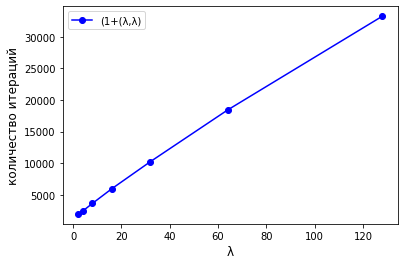
\includegraphics[scale=1]{Lambda}}
\caption{Производительность \ollga для различных значений $\lambda$ на полных графах с числом вершин $2^{10}$.}
\label{fig:lambda}
\end{figure}

На Рисунке~\ref{fig:lambda} изображен график зависимости числа вычислений функции приспособленности от значий $\lambda$. Исходя из графика, можно сделать вывод, что брать большую $\lambda$ не оптимально, но и в случае слишком маленького значения, например равному единице, алгоритм не будет отличаться от \oea. Тогда, чтобы была возможность оценить эффективность данного генетического алгоритма, выберем $\lambda = 10$. Для всех запусков \alglambdaf использовалась именно эта константа.

Для каждого запуска на каждой итерации собиралась и записывалась  информация:
\begin{itemize}
 \item текущее значение функции приспособленности $f$;
 \item значение $f$ для победителя мутации;
 \item значение $f$ для победителя скрещивания (для \alglambdaf).
\end{itemize}

Такой сбор информации позволяет более детально увидеть и проанализировать работу алгоритма на практике.
Также после завершения каждого алгоритма фиксировалось число вычислений функции приспособленности.
Реализация всех описанных выше алгоритмов предоставлена в виде программы на языке C++ в Приложении~\ref{ollgaStat}

\section{Сравнение эмпирической и теоретической оценок на полных графах}

Рассмотрим полученные результаты для полных графов и посмотрим как разные эволюционные алгоритмы решают задачу о максимальном разрезе графа на практике.
Для них в предыдущей главе уже получена теоретическая оценка.
Напомним, что для RLS оценка числа вычислений функций приспособленности до достижения оптимума $nln2 - o(n)$, для \oea со стандартным оператором мутации --- $enln2 - o(n)$, \oea с оператором мутации с выбором мутации по степенному закону --- $\Theta(n^{\beta-1})$, но так как для экспериментов использовалась $\beta$ равная $1,5$, ожидаемое время $\Theta(\sqrt{n})$, и для \alglambdaf --- $O\left(\frac{\lambda n\ln \ln \lambda}{\ln \lambda}\right)$.

\begin{figure}[t!]
\center{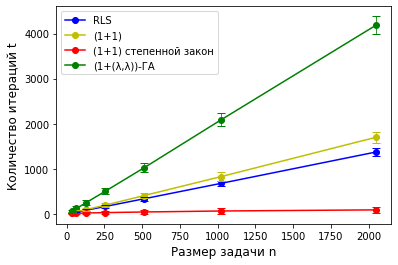
\includegraphics[scale=1]{KN}}
\caption{Графики зависимости времени работы эволюционных алгоритмов на полных графах от размера задачи.}
\label{fig:kn}
\end{figure}

Сравним полученные теоретическую и эмпирическую оценку.
На Рисунке~\ref{fig:kn} изображен график зависимости числа вычислений функции приспособленности до нахождения искомого приближения оптимума от числа вершин.
Сразу можно заметить, что алгоритмы Random Local Search и \oea работают схожим образом.
Это связано с тем, что RLS на каждой своей итерации инвертирует один бит и ожидаемое число инвертированных битов в (1+1) так же равно единице. В реальности еще существуют итерации, создающие точную копию родительской особи, что ухудшает работу алгоритма.
Алгоритм (1+1) с распределением с <<тяжелым хвостом>> показал наилучший результат, как и ожидалось. Такой алгоритм движется к оптимуму суперконстантными шагами, так как может заменить сразу много символов с гораздо большей вероятностью. В нашей задаче больше половины битов нули, поэтому выгодно инвертировать много битов, соответственно этот алгоритм работает значительно лучше чем RLS и (1+1) со стандартным типом мутации. Судя по графику, эмпирическая оценка близка к константной.

Что касаемо алгоритма \alglambdaf, он показал свою неэффективность на данной задаче. Согласно полученным результатам \alglambdaf не дает преимущество над тривиальными алгоритмами. Как минимум из-за дополнительных $2\lambda$ вычислений функции приспособленности на каждой итерации алгоритма.
Отклонение времени работы \alglambdaf от среднего составляет около $10\%$, что также изображено на графике.

\section{Результаты экспериментов на разных типах графов}

\begin{figure}[t!]
\center{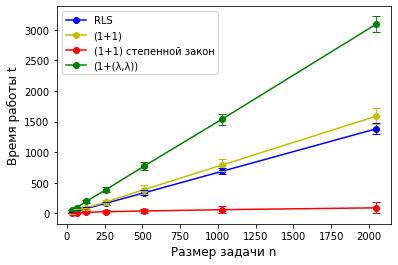
\includegraphics[scale=1]{KNN}}
\caption{Графики зависимости времени работы эволюционных алгоритмов на полных двудольных графах от размера задачи.}
\label{fig:knn}
\end{figure}

\begin{figure}[t!]
\center{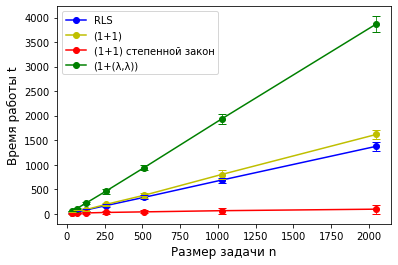
\includegraphics[scale=1]{Random}}
\caption{Графики зависимости времени работы эволюционных алгоритмов на случайных графах от размера задачи.}
\label{fig:rand}
\end{figure}

Проанализируем, как алгоритмы находят решение, где половина ребер <<разрезана>>, на полных двудольных и случайных графах.
Для полных двудольных графов такое условие остановки алгоритма дает результат в два раза хуже, чем наилучший, так как в таких графах можно разрезать все ребра.
Для случайно сгенерированных графов мы не можем знать заранее, насколько полученный ответ близок к оптимальному.
И в отличие от описанного ранее анализа алгоритмов на полных графах, не можем оценить ожидаемое число единиц в искомом разбиении.

На Рисунках~\ref{fig:knn} и~\ref{fig:rand} изображены графики зависимости числа вычислений функции приспособленности от размера задачи для полных двудольных и случайных графов соответственно.

Результаты экспериментов схожи с результатами на полных графах. Генетический алгоритм \alglambda все еще не показал свою эффективность по сравнению с другими эволюционными алгоритмами.
Заметим, что алгоритм \oea с оператором мутации с выбором вероятности по степенному закону показал наилучший результат и на других типах графов.
Исходя из проведенных экспериментов, можно сделать вывод, что алгоритмы работают схожим образом, как и на полных графах, и предполагаемое время работы \alglambdaf на задаче максимального разреза графа на всех типах графов --- $O\left(\frac{\lambda n\ln \ln \lambda}{\ln \lambda}\right)$.



\chapterconclusion
В этой главе были проанализированы результаты запусков эволюционных алгоритмов на задаче поиска максимального разреза графа для различных типов графов. Полученная эмпирическая оценка соответствует ожиданиям, полученным во 2 главе.
Также на основании полученных результатов проведенных экспериментов можно предполагать, что ожидаемое время работы \alglambdaf для разных типов графов такое же, как и для полных, и равно $O\left(\frac{\lambda n\ln \ln \lambda}{\ln \lambda}\right)$.

\finishrelatedwork

%% Макрос для заключения. Совместим со старым стилевиком.
\startconclusionpage
В данной работе была проанализирована работа генетического алгоритма \alglambda на задаче поиска максимального разреза графа. Для полных графов была получена теоретическая оценка ожидаемого числа вычислений функции приспособленности, равная $O\left(\frac{\lambda n\ln \ln \lambda}{\ln \lambda}\right)$, а также проведено сравнение с другими эволюционными алгоритмами.
Проанализировано время работы алгоритмов на задаче максимального разреза графа на практике.
Из полученных в данной работе результатов можно сделать вывод о неэффективности выбора \alglambdaf на данной задаче.

Для продолжения работы по этой теме и дополнительных оценок \alglambdaf на задаче поиска максимального разреза графа можно провести исследования в области подбора параметров, которые улучшат эффективность алгоритма, а также различные модификации операторов мутации и скрещивания.

\printmainbibliography

%% После этой команды chapter будет генерировать приложения, нумерованные русскими буквами.
%% \startappendices из старого стилевика будет делать то же самое
\appendix


\end{document}
